%%%%%%%%%%%%%%%%%%%%%%%%%%% Figure 13 FjordOs salinity %%%%%%%%%%%%%%%%%%%%
\begin{figure}[t]
 \begin{center}
  \begin{pspicture}(0,0)(15,12)
   \rput[b]( 7.5,0.0){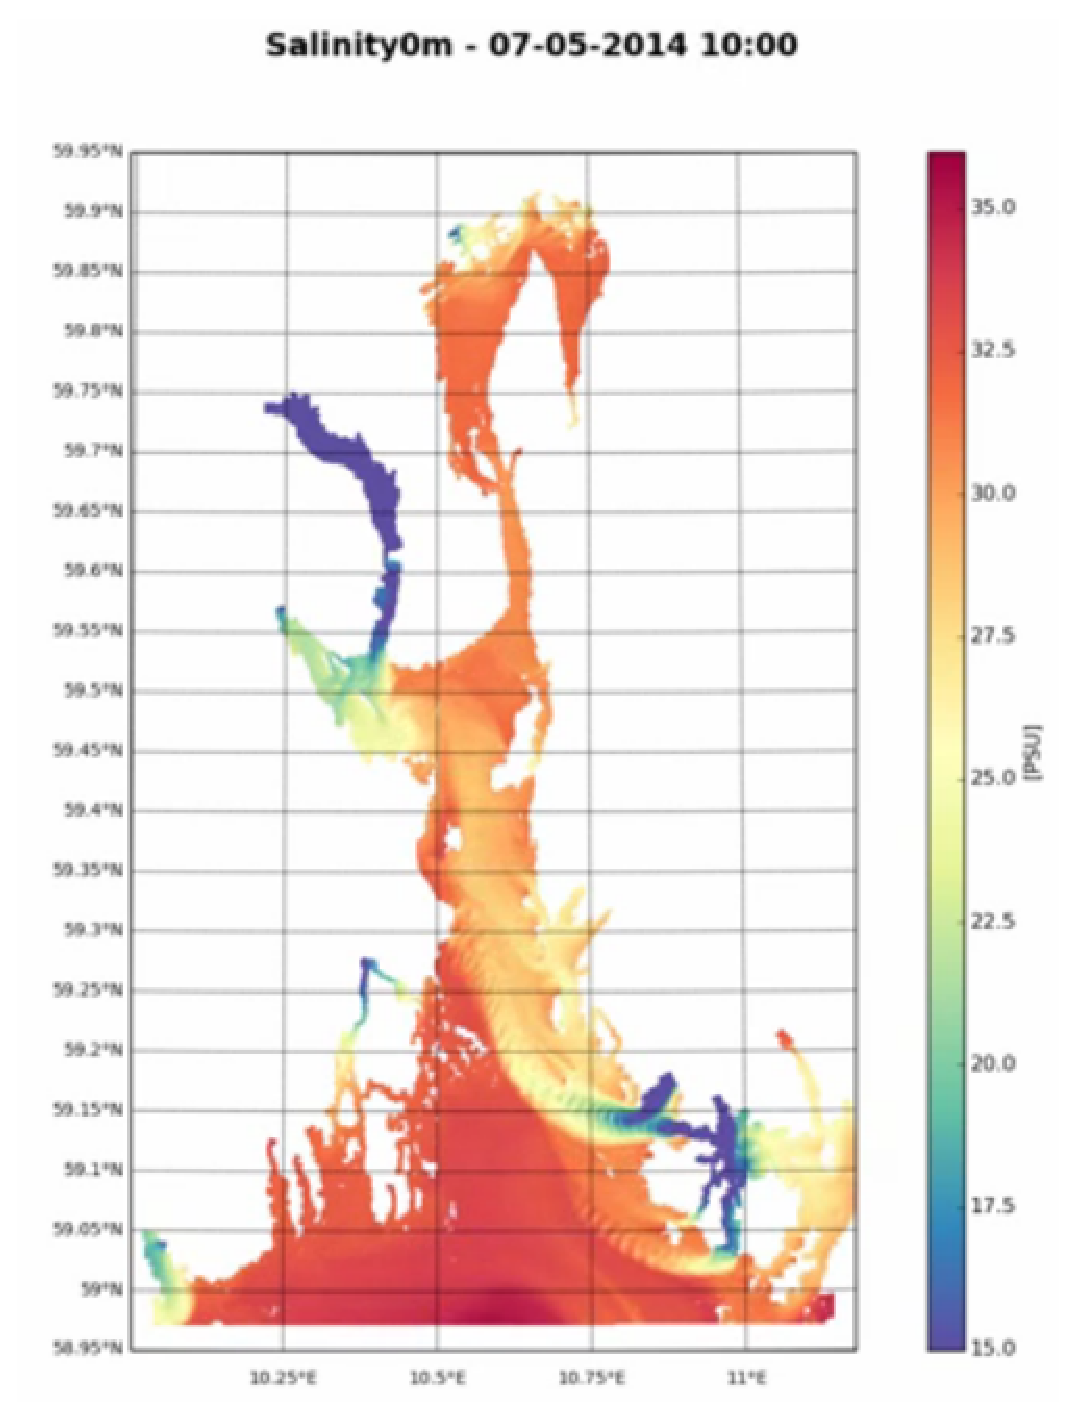
\includegraphics[height=12cm]{fjordos_salinity}}
  \end{pspicture}
  \caption{\small Daily mean sea surface salinity valid at May 7, 2014 from an earlier testrun. The color bar gives salinity in units of psu. Longitude and latitude are indicated along the axes. Note the impact of the freshwater discharged by the major rivers on the salinity, and the tendency of the Coriolis effect to turn the freshwater flux from Glomma northward.} 
  \label{fig:fjordos_salinity}
 \end{center}
\end{figure}

